\section{Neural Network Types}
\label{sec:nnet_types}

\subsection{Feed Forward Neural Networks (Multilayer Perceptron)}

Structure of perceptron make a way for feed forward neural layers. 
Unlike stated above, a neural layer might output multiple values (say $o \in \mathbb{R}^{1 \times d_o}$) as vector from input (say $x \in \mathbb{R}^{1 \times d_x}$). 
Such a setting forces parameter $W \in \mathbb{R}^{d_x \times d_o} $ to be a matrix. 
Moreover, activation function is not necessariliy step function. 
It can be any nonlinear function like sigmoid, tanh, ReLU etc. 
Feed Forward Neural Networks are generalization of perceptron to approximate any function $f^*$. 
Neural layers are stacked to construct deep feed forward neural network. 
It defines a nonlinear mapping $y=f(x;\theta)$ between input $x$ and output $y$, parametrized by $\theta$ which is set of all learnable parameters like weights, bias and other possible values.

Assuming input signal is $x \in \mathbb{R}^{1 \times d_x}$ (output of previous layer), 
activation value of the layer ($h \in \mathbb{R}^{d_x \times d_h}$) is evaluated as by linear transformation followed by nonlinear activation, 
\begin{equation}
\label{eqn:mlpact}
h = f (x W + b),
\end{equation}
where activation $f$ is applied elementwise.

\subsection{Residual Feed Forward Neural Networks}

As Feed Forward Networks becomes deeper, optimizing weights gets difficult. 
Therefore, people come with the idea of residual connections~\cite{he_deep_2015}. 
For a fixed number of stacked layers (usually 2), input and output of the stack is summed up for next calculations. 
Replacing feed forward layers with other types yield different kind of residual network. 
The difference is demonstrated in \figref{fig:rffnn_ffnn}. 

\begin{figure}
	\centering
	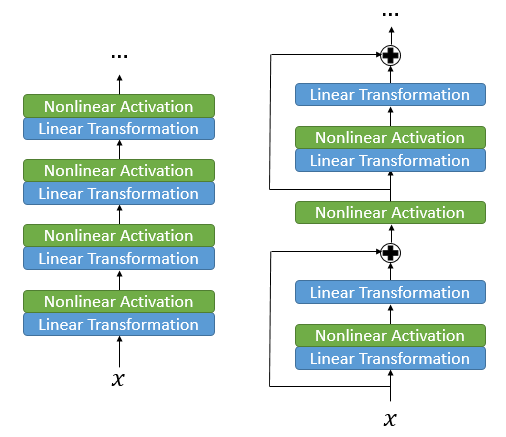
\includegraphics[width=0.5\textwidth]{figures/ml_theory/rffnn_ffnn.png}
	\caption{Deep Feed Forward (left) and Deep Residual Feed Forward Network (right)}
	\label{fig:rffnn_ffnn}
\end{figure}

\subsection{Recurrent Neural Networks}

Recurrent Neural Networks (RNNs) \cite{rumelhart_learning_1986} are type of neural network to process sequential data. 
It is specialized for data having sequential topology. 
It is used commonly used for sequence based applications. 

In FFNN layer, output only depends on its input, while Recurrent Layer output is dependent on both input at time $t$ and its output in previous time step $t-1$. 

RNN can be thought as multiple copies of same network which passes message to its successor through time. 
A RNN layer is similar to FFNN layer as in \eqref{eqn:mlpact}, 
except input is concatenation of output feedback and input itself.

Given input sequence $x \in \mathbb{R}^{T \times d_x}$, ,output sequence $h \in \mathbb{R}^{T \times d_h}$ is evaluated recursively,  
\begin{equation}
\label{eqn:rnnact}
h_t = f (h_{t-1} \tilde{W} + x_t W + b)
\end{equation}
where nonlinear activation $f$ \ref{eqn:mlpact} applied element-wise again. Initial output $h_0$ can be either parametrized or assigned as zeros vector. A comparison between FFNN and RNN layer is visualized in \figref{fig:rnn_vs_ffnn}

\begin{figure}
	\centering
	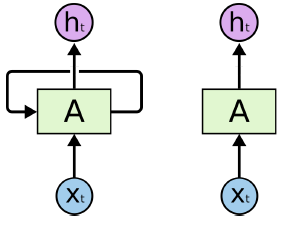
\includegraphics[width=0.5\textwidth]{figures/ml_theory/rnn_vs_ffnn_layer.png}
	\caption{Recurrent Layer (left) and Feed Forward Layer (right) illustration.}
	\label{fig:rnn_vs_ffnn}
\end{figure}

\subsubsection{Long Short Term Memory}

Conventional RNNs have problem with vanishing/exploding gradient problem \cite{olah_understanding_2015}. 
As the sequence gets longer, effect of initial inputs in sequence decreases. 
This causes long term dependence problem. 
If information from initial inputs required, gradients either vanish or explode. 
In order to overcome this problem another architecture is developed called Long Short Term Memory (LSTM)~\cite{hochreiter_long_1997}. 

LSTM is a special type of RNN. 
It is explicitly designed to allow learning long-term dependencies. 
A single LSTM cell has 4 neural layer while vanilla RNN layer has only one neural layer. 
In addition to hidden state $h_t$, there is another state called cell state $C_t$. 
Information flow is controlled by 3 gates. 

\begin{figure}
	\centering
	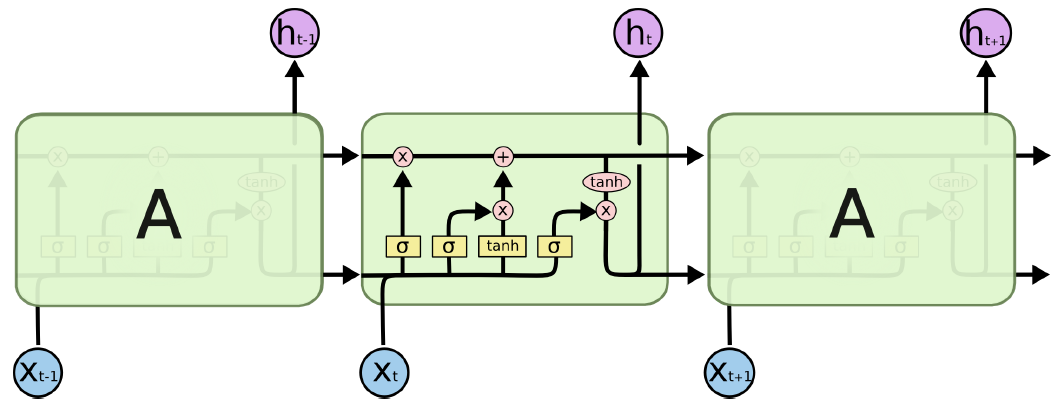
\includegraphics[width=0.98\textwidth]{figures/ml_theory/lstm/lstm_module.png}
	\caption{LSTM Cell}
	\label{fig:lstm_cell}
\end{figure}

\textbf{Forget Gate} controls past memory. 
According to input, past memory is either kept or forgotten. 
Sigmoid function ($\sigma$) is used as activation function, applied elementwise. Mathematically, 
\begin{equation}
\label{eqn:lstm_forget}
f_t = \sigma( [h_{t-1}; x_t] W_f + b_f).
\end{equation}

Hyperbolic tangent layer creates new candidate of cell state from input, 
\begin{equation}
\label{eqn:lstm_cellstcand}
\hat{C}_t = \tanh( [h_{t-1}; x_t] W_C + b_C).
\end{equation}

\textbf{Input Gate} controls contribution from input to cell state (memory), 
\begin{equation}
\label{eqn:lstm_inp}
i_t = \sigma( [h_{t-1}; x_t] W_i + b_{i}).
\end{equation}
Once what are to be forgotten and added decided, cell state is updated as
\begin{equation}
\label{eqn:lstm_cellstupt}
C_t = f_t \odot C_{t-1} + i_t \odot \hat{C}_t.
\end{equation}
using input gate and forget gate outputs.

\textbf{Output Gate} controls which part of new cell state to be output as
\begin{equation}
\label{eqn:lstm_out}
o_t = \sigma( [h_{t-1}; x_t] W_o + b_o).
\end{equation}

Lastly, cell state is filtered by tanh to push values to be in $(-1,1)$ before evaluating hidden state $h_t$ using output gate outputs,
\begin{equation}
h_t = o_t \odot \tanh(C_t).
\end{equation}

\subsection{Attention Mechanism}

As stated earlier, recurrent neural networks are prone to forget long term dependencies. 
LSTM and other variants are invented to overcome this problem. 
Although they reduced this, they cannot attend specific parts of the input. 
Therefore, people came with the idea of weighted averaging all states through time where weights depends on both input and output. 
Assume that input sequence $x \in \mathbb{R}^{T \times d_X}$ is encoded to $h \in \mathbb{R}^{T \times d_H}$. 
The context vector is calculated using weight vector $\alpha \in \mathbb{R}^{1 \times T}$,
\begin{equation}
\mathrm{Attention}(q, h) = \alpha h. %\sum_{\tau=1}^{T} \alpha_{\tau} h_{\tau}.
\label{eq:attention_generic}
\end{equation}

Calculation of weight vector depends on the task. 
For each time step, a score function is calculated between hidden state $h \in \mathbb{R}^{T \times d_H}$ and query $q$ (which may be many things depending on task). 
Attention score is $\alpha \in \mathbb{R}^{T}$ is calculated using predefined arbitrary function $f$ depending on choice. In general form,  
\begin{equation}
\alpha = f(q, h; \theta_{score}).
\end{equation}

\subsubsection{Transformer}

The Transformer was proposed in Attention is All You Need~ \cite{vaswani_attention_2017} paper. 
Unlike recurrent networks, this architecture is solely builded on attention layers. 

A transformer layer consists of feed-forward and attention layers, which makes the mechanism special. 
Like RNNs, it can be used as both encoder and decoder. 
While encoder layers attend to itself, decoder layers attends both itself and encoded input. 

\textbf{Attention Layer} is a mapping from 3 vectors called query $Q \in \mathbb{R}^{T \times d_k}$, key $K \in \mathbb{R}^{T \times d_k}$ and value $V \in \mathbb{R}^{T \times d_v}$ to output, 
where $T$ is time length, $d_k$ and $d_v$ are embedding dimensions. 
Output is weighted sum of values $V$ while weights are evaluated by compatibility metric of query $Q$ and key $K$. 
In vanilla transformer, compatibility of query and key is evaluated by dot product, normalizing by $\sqrt{d_k}$. 
For a query, dot product with all keys are evaluated, then softmax function is applied to get weights of values. Mathematically, 
\begin{equation}
\mathrm{Attention}(Q, K, V) = \mathrm{softmax}(\frac{Q^{T}. K}{\sqrt{d_k}}) V
\end{equation}
This approach is called Scaled Dot-product Attention. 

Instead of performing single attention, \textbf{Multi-Head Attention} projects keys, queries and values linearly from $d_m$ dimensional vector space to $h$ different spaces using projection matrices. 
Then, attention is done $h$ times, and results are then concatenated and linearly projected to final values of the layer.
Projection matrices are model parameters, $W^Q_i \in \mathbb{R}^{d_m \times d_k}$, $W^K_i \in \mathbb{R}^{d_m \times d_k}$, $W^V_i \in \mathbb{R}^{d_m \times d_v}$ for $i=1,...,h$. 
Also output matrix is used to project multiple values into single one, $W^O \in \mathbb{R}^{h d_v \times d_m}$. Mathematically, 
\begin{equation}
\begin{split}
% It is better to write these as \DeclareMathOp
\mathrm{MHA}(Q,K,V) &=  \text{Concat}(\mathrm{head}_1, \mathrm{head}_2, ... \mathrm{head}_h)W^O \\
\mathrm{head}_i &=  \text{Attention}(QW^Q_i,KW^K_i,VW^V_i)
\end{split}.
\end{equation}

Both encoder and decoder contains \textbf{Feed Forward Layer}, containing two linear transformations with ReLU activation.
\begin{equation}
\mathrm{FFN}(x) = \text{ReLU}(xW_1+b)W_2+b_2
\end{equation}

\textbf{Encoder Layer} starts with a residual self attention layer. 
Self attention means that query, key and value are same vectors. 
Then it is followed by feed forward neural layer. 
Both sublayers are employed with resudial connection with layer normalization, 
i.e summation of layer input and output is passed through layer normalization. 
\begin{equation}
\begin{split}
a = & \mathrm{LN}(x + \mathrm{MHA}(x,x,x)) \\
y = & \mathrm{LN}(a + \mathrm{FFN}(att))
\end{split}
\end{equation}

\textbf{Decoder Layer} has also self-attention and feed forward layers similar to encoder layer. 
In addition, there is another attention layer which is over encoder outputs. 
Same as encoder, all sublayers have resudial connection with layer normalization. 
Let's call encoded sequence $e \in \mathbb{R}^{T \times d_m}$ and decoded sequence $d \in \mathbb{R}^{T \times d_m}$ (masked). 
Assume that the sequence decoded up to $t$th point in sequence. 
Then, $d_{t+1}$ is calculated as follows. 
\begin{equation}
\begin{split}
a = & \mathrm{LN}(d_{1:t}+\mathrm{MHA}(d_{1:t},d_{1:t},d_{1:t})) \\
s = & \mathrm{LN}(att+ \mathrm{MHA}(a,e,e)) \\
d_{t+1} = & \mathrm{LN}(s+ \mathrm{FFN}(s))
\end{split}
\end{equation}

Since there are no recurrent or convolutional architecture in the model, sequential information needs to be embedded. 
For this purpose, \textbf{Positional encoding}s are used. 
They have same dimension with input $x$, so that input embeddings can be added to at the beginning of encoder or decoder stacks. 
For position $p$, $2i$ or $2i+1$th dimension has following values ($i \in \mathbb{N}$), 
\begin{equation}
\begin{split}
\mathrm{PE}_{p,2i} = \sin(pos/10000^{2i/d_m}) \\
\mathrm{PE}_{p,2i+1} = \cos(pos/10000^{2i/d_m})
\end{split},
\end{equation}
as proposed in the original paper. 

\subsubsection{Pre-Layer Normalized Transformer}

Original transformer architecture includes layer normalization operations after attention and feed-forward layers. 
It is unstable since gradients of output layers are high, so Pre-Layer Normalized transformer is proposed by \cite{xiong_layer_2020} by carrying layer normalization operation to in front of attention and feed-forward layers. 
Moreover, Parisotto et al. Xiong et al.~ \cite{parisotto_stabilizing_2019} proposed gated transformer which also includes layer normalizations before attention and feedforward layer. 
They also stated that although gated architecture improves many RL tasks drastically, non-gated pre-layer normalized transformer are good enough. 

In pre-layer normalized transformer, encoder equations are as follows,
\begin{equation}
\begin{split}
att = & x+ \mathrm{MHA}(\mathrm{LN}(x),\mathrm{LN}(x),\mathrm{LN}(x)) \\
y = & att+ \mathrm{FFN}(\mathrm{LN}(att))
\end{split}.
\end{equation}
The difference between post-layer and pre-layer transformer encoders are visualized in \figref{fig:post_pre_trsf}

\begin{figure}
	\centering
	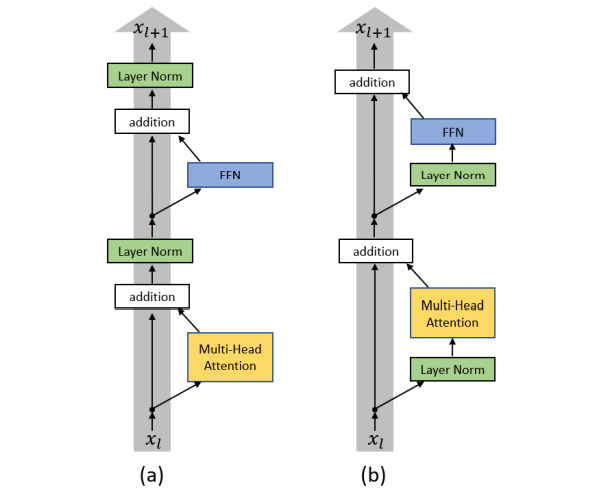
\includegraphics[width=0.55\textwidth]{figures/ml_theory/post_pre_trsf.png}
	\caption{(a) Post-LN Transformer layer, (b) Pre-LN Transformer
		layer.}
	\label{fig:post_pre_trsf}
\end{figure}

%Decoder equations are as follows.
%\begin{equation}
%\begin{split}
%att = & %d_{1:t}+\mathrm{MHA}(\mathrm{LN}(d_{1:t}),\mathrm{LN}(d_{1:t}),\mathrm%{LN}(d_{1:t})) \\
%dec = & att+ \mathrm{MHA}(\mathrm{LN}(att),\mathrm{LN}(att),\mathrm{LN}(att)) \\
%d_{t+1} = & dec+ \mathrm{FFN}(\mathrm{LN}(dec))
%\end{split}
%\end{equation}

